



\chapter{Fundamentação Teórica}

\section{Processamento Digital de Imagens}

Processamento digital de imagens segundo \citeonline{jain1989fundamentals}, consiste na manipulação de imagens em formato digital utilizando algoritmos para extrair informações, melhorar a qualidade ou transformar dados visuais. Esta área engloba diversas técnicas que permitem o tratamento de imagens capturadas por dispositivos digitais, como câmeras e scanners, visando a otimização de aspectos como contraste, nitidez e remoção de ruído \cite{gonzalez2010processamento}. Além de aprimorar a percepção visual, essas técnicas são essenciais para a análise automática de imagens, facilitando a identificação e classificação de objetos, a medição de propriedades geométricas e a extração de padrões \cite{russ2006image}.

No processamento digital de imagens, os processos geralmente são abordados em três níveis distintos, cada um com um papel específico na análise e interpretação das imagens. O nível baixo trata de manipulações mais primitivas, realizando operações fundamentais como filtragem, aprimoramento de contraste e remoção de ruído. O nível médio foca na segmentação e extração de características, onde a imagem é dividida em regiões de interesse e características relevantes são identificadas e descritas. Finalmente, o nível alto envolve a interpretação e reconhecimento dos dados processados, onde algoritmos são aplicados para classificar objetos, reconhecer padrões e realizar decisões baseadas em informações extraídas dos níveis anteriores. Cada um desses níveis do processamento de imagens contribui de maneira distinta para a análise visual, formando uma cadeia de processamento que vai desde a manipulação básica até a interpretação complexa \cite{gonzalez2010processamento}. 

Ainda segundo \citeonline{gonzalez2010processamento} o processamento digital de imagens envolve uma série de passos que vão desde a aquisição até interpretação das imagens. Como pode ser visto na Figura \ref{etapasProcessamentoImagens}, essas etapas incluem:


\begin{enumerate}
    \item \textbf{Aquisição de Imagem}: Este estágio trata da obtenção de imagens, que podem ser capturadas por dispositivos digitais ou provenientes de arquivos digitais já existentes. Neste processo, podem ser realizados ajustes iniciais, como modificar o tamanho da imagem.
    
    \item \textbf{Filtragem e realce de imagens}: Nesta fase, a imagem é manipulada para adequá-la a uma aplicação específica. Em alguns casos, como em imagens médicas, a melhoria pode não ser a abordagem mais apropriada.

    \item \textbf{Restauração de imagens}: Este passo busca aprimorar a qualidade visual das imagens através de métodos baseados em modelos matemáticos ou probabilísticos para compensar a degradação da imagem.

    \item \textbf{Processamento de Imagens em Cores}: Com o aumento do uso de imagens digitais na web, o processamento de imagens coloridas tornou-se fundamental. Trabalhar com cores facilita a extração de características relevantes de uma imagem.

    \item \textbf{Processamento em Multiresolução}: Este método envolve a representação de uma imagem em diferentes níveis de resolução, permitindo uma análise detalhada em várias escalas.

    \item \textbf{Compressão de Imagem}: Nesta fase, são aplicadas técnicas para armazenar imagens de maneira mais eficiente ou reduzir a largura de banda necessária para sua transmissão.

    \item \textbf{Processamento Morfológico}: O processamento morfológico foca na extração e análise dos componentes da imagem para descrever suas formas.

    \item \textbf{Segmentação}: A segmentação é um dos aspectos mais desafiadores no processamento digital de imagens. Ela consiste em dividir a imagem em partes ou objetos distintos.

    \item \textbf{Representação e Descrição de Características}: Este processo, também conhecido como seleção de atributos, visa extrair características que forneçam informações quantitativas ou qualitativas para distinguir entre diferentes tipos de objetos.

    \item \textbf{Identificação de Objetos}: O reconhecimento de objetos é o processo de atribuir rótulos a elementos presentes em uma imagem, como classificar um objeto como um "carro".

    \item \textbf{Base de conhecimento}: Envolve o entendimento do domínio do problema, incluindo informações detalhadas sobre áreas específicas na imagem onde se espera encontrar dados relevantes.

    
\end{enumerate}

\begin{figure}
    \centering   
    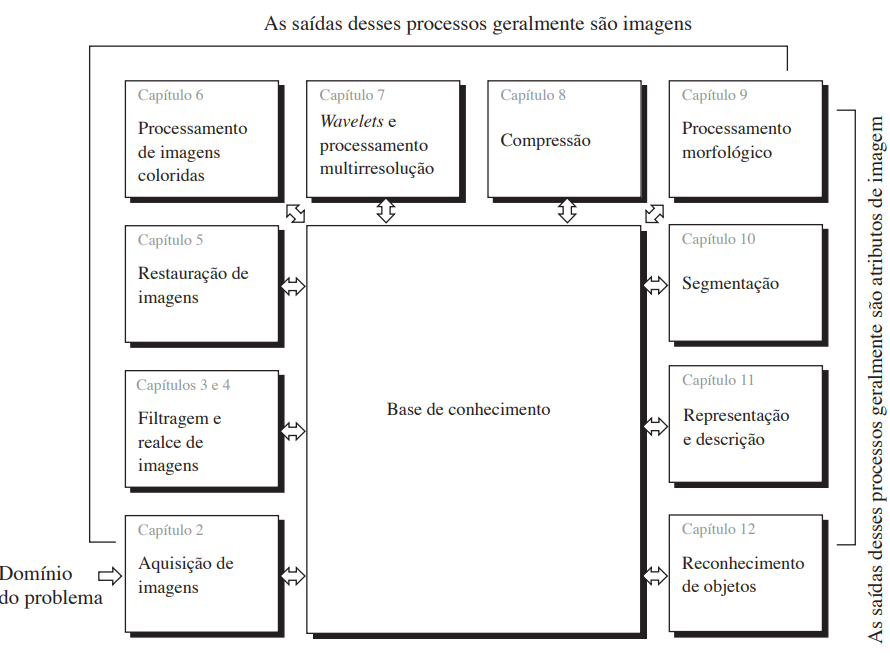
\includegraphics[width=\textwidth]{fig/PassosProcessamentoDigitalDeImagens.png}
    \caption{Etapas do processamento digital de imagens que vai desde a aquisição de imagens até a identificação e descrição de objetos presente nelas.}
    \label{etapasProcessamentoImagens}
\end{figure}

O processamento digital de imagens é amplamente aplicado em áreas como a medicina, para a análise de imagens de diagnóstico, na indústria, para o controle de qualidade de produtos, na segurança, para reconhecimento facial e monitoramento e entre outros \cite{gonzalez2010processamento}. %https://archive.org/details/imageprocessingh03edruss




\subsection{Transformação de Intensidade}


As transformações de intensidade são técnicas no processamento digital de imagens focadas na manipulação direta dos valores de intensidade dos pixels. Elas operam individualmente em cada pixel, possibilitando ajustes de contraste, brilho e outros atributos de uma imagem. O objetivo principal dessas transformações é modificar a aparência visual da imagem para realçar características específicas ou preparar a imagem para análises posteriores \cite{gonzalez2010processamento}.

% No processamento digital, cada pixel de uma imagem é representado por um valor de intensidade, que pode ser ajustado através de uma transformação matemática. A relação entre os valores de intensidade antes e depois da transformação é descrita pela função $s=T(r)$, onde $r$ é o valor de intensidade original, $s$ é o valor de intensidade transformado, e $T$ é a função de transformação. Esses valores são manipulados usando tabelas indexadas, especialmente em ambientes de 8 bits, onde a tabela contém 256 entradas para mapear os valores de $r$ em $s$.

% gonzales pag 55 e 69 operações basicas da transformação de intensidade
As principais funções de transformação de intensidade incluem:

\textbf{Transformações Lineares:} Essas funções incluem transformações como o negativo e a identidade. A transformação de negativo inverte os valores de intensidade, enquanto a identidade mantém os valores de intensidade inalterados.

\textbf{Transformações Logarítmicas:} Essas funções utilizam operações logarítmicas para alterar a distribuição de intensidade. Transformações como o logaritmo e o logaritmo inverso são utilizadas para melhorar detalhes em áreas escuras da imagem ou para estender o alcance dinâmico.

\textbf{Transformações de Potência:} Utilizam funções de potência e raiz para ajustar o contraste e a gama da imagem. Transformações de n-ésima potência e n-ésima raiz são exemplos de como essas funções podem ajustar as características da imagem.

Assim, ao aplicar transformações de intensidade e técnicas de filtragem, é possível ajustar e melhorar imagens de maneira significativa, seja para visualização aprimorada ou para análises mais precisas.
% EXEMPLO optional
Considere a transformação de intensidade ilustrada na Figura \ref{exemploTransformacaoIntensidade}.a. Como mostra \citeonline{gonzalez2010processamento}, quando aplicamos essa transformação a cada pixel da imagem original $f$, geramos uma nova imagem $g$ com maior contraste. Nesta transformação, os valores de intensidade abaixo de um ponto $k$ são escurecidos, enquanto os valores acima de $k$ são clareados. Isso resulta em uma imagem com contraste ampliado, onde áreas escuras são mais densas e áreas claras são mais evidentes.

Na Figura \ref{exemploTransformacaoIntensidade}.b, a transformação $T(r)$ resulta em uma imagem binária, onde os pixels são convertidos em apenas dois níveis de intensidade, dependendo de um limiar específico. Essa técnica, conhecida como limiarização, simplifica a imagem original em uma forma mais clara e destacada, com apenas duas cores, tipicamente preto e branco.

Essas transformações são exemplos de como ajustes nos valores de intensidade podem alterar significativamente a aparência e a utilidade da imagem, dependendo do objetivo do processamento.

\begin{figure}
    \centering   
    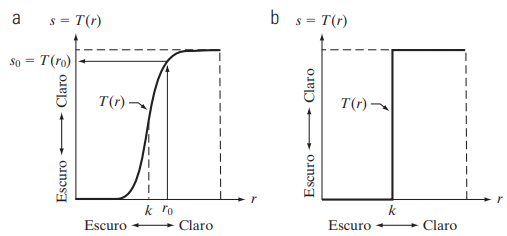
\includegraphics[width=\textwidth]{fig/ExemploTranformacaoIntensidade.png}
    \caption{Funções para ajuste da intensidade em imagens. (a) Método de ampliação de contraste, que aumenta a diferença entre os níveis de intensidade, destacando áreas mais escuras e mais claras. (b) Método de binarização, que converte a imagem em dois níveis distintos de intensidade, geralmente preto e branco, com base em um limiar definido.}
    \label{exemploTransformacaoIntensidade}
\end{figure}


\section{Deep Learning}

Deep Learning, ou Aprendizado Profundo, é uma subárea do aprendizado de máquina que se concentra em redes neurais artificiais com muitas camadas (ou "profundidade"). Estas redes neurais são projetadas para simular o funcionamento do cérebro humano e aprender representações de dados em múltiplos níveis de abstração \cite{goodfellow2016deep}.
As redes neurais profundas, são compostas por múltiplas camadas de neurônios artificiais. Cada camada da rede realiza uma transformação não linear sobre os dados, permitindo à rede aprender representações complexas e hierárquicas dos dados de entrada \cite{haykin2001redes}.

%https://books.google.com.br/books?id=ig8mHog30X0C&lpg=PA398&ots=fnfB2Z7MCV&dq=perceptron%20Rosenblatt&lr&hl=pt-BR&pg=PA398#v=onepage&q=perceptron%20Rosenblatt&f=false % evolucao 
O campo das redes neurais evoluiu significativamente desde suas primeiras iterações. Um marco importante nesse desenvolvimento foi o trabalho de \citeonline{rosenblatt2021perceptron}, que introduziu o perceptron na década de 1960. Essa técnica inicial mostrou que, sob certas condições, um perceptron poderia aprender a classificar dados linearmente separáveis, mas enfrentava limitações com problemas mais complexos.
A real revolução no campo das redes neurais veio com o desenvolvimento de redes neurais de múltiplas camadas. Em 1986, \citeonline{rumelhart19881986} introduziram o algoritmo de retropropagação, também conhecido como a regra delta generalizada. Este método permitiu o treinamento eficaz de redes neurais com várias camadas, superando as limitações dos perceptrons simples e proporcionando um avanço significativo no desempenho e na aplicabilidade das redes neurais.

% No nível mais básico, o perceptron é uma rede neural que aprende a tomar decisões lineares, ou seja, ele divide os dados em duas classes distintas com base em uma função de decisão linear. No entanto, redes neurais mais avançadas, como as redes neurais profundas, são capazes de modelar relações complexas e não lineares em dados, permitindo aplicações sofisticadas em áreas como reconhecimento de imagem, processamento de linguagem natural e muito mais. // escrevi e ficou nada ver

O perceptron é uma das estruturas fundamentais das redes neurais, representando o modelo mais simples de um neurônio artificial. Introduzido por \citeonline{rosenblatt2021perceptron}, o perceptron é capaz de realizar classificações binárias, distinguindo entre duas classes distintas com base em dados de entrada.

Um perceptron funciona através de uma série de operações matemáticas simples. Inicialmente, cada entrada é multiplicada por um peso, que é um valor numérico associado a essa entrada. Esses pesos são ajustados durante o processo de treinamento para que o perceptron aprenda a mapear as entradas para as saídas desejadas. A soma ponderada dessas entradas é então calculada e passada por uma função de ativação, que decide se o neurônio "ativa" ou não. Tradicionalmente, a função de ativação usada em um perceptron simples é a função degrau, que retorna um valor binário - geralmente 0 ou 1 \cite{hertz2018introduction}. Esse processo pode ser formalmente expresso pela fórmula:

\[
y = f\left(\sum_{i=1}^{n} w_i x_i + b\right)
\]

onde $y$ é a saída do perceptron, $x_i$ são as entradas, $w_i$ são os pesos associados, $b$ é o bias (um termo adicional que permite que o modelo ajuste a função de ativação, mesmo com todas as entradas em zero), e $f$ é a função de ativação.

A Figura \ref{fig:perceptron} ilustra visualmente a estrutura de um perceptron, mostrando as entradas, pesos, soma ponderada, bias, função de ativação e uma saída.

\begin{figure}
    \centering   
    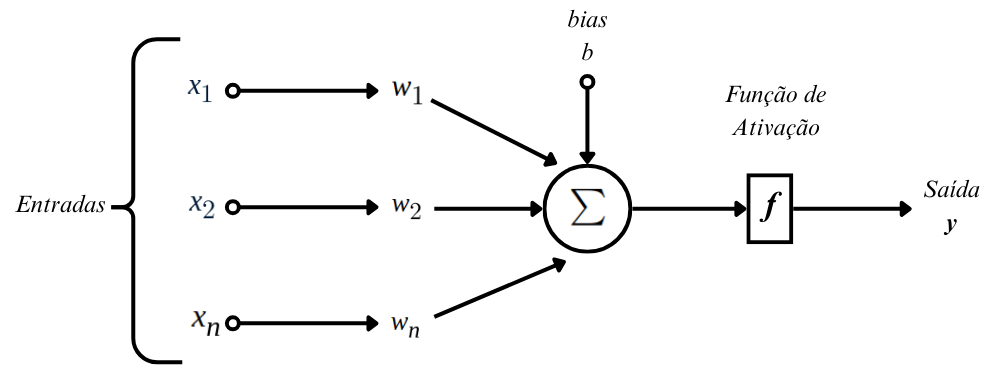
\includegraphics[width=0.7\textwidth]{fig/perceptron.png}
    \caption{Diagrama de um perceptron, ilustrando uma abordagem simplificada baseada na estrutura e função de um neurônio biológico.}
    \label{fig:perceptron}
\end{figure}

O perceptron aprende a partir de um processo de ajuste de pesos, conhecido como regra de aprendizagem do perceptron. Durante o treinamento, o perceptron ajusta os pesos com base no erro da saída prevista em relação à saída desejada. Esse ajuste é feito através de um processo iterativo, onde o erro é propagado de volta através da rede e os pesos são atualizados para minimizar o erro, seguindo a equação:

\[
w_i = w_i + \Delta w_i
\]

\[
\Delta w_i = \eta (d - y) x_i
\]

onde \( \Delta w_i \) é o ajuste do peso, \( \eta \) é a taxa de aprendizado, \( d \) é a saída desejada, e \( y \) é a saída calculada pelo perceptron. A taxa de aprendizado é um parâmetro importante que controla o quão rapidamente o modelo se adapta aos dados.

Embora o perceptron tenha sido um avanço significativo na época de sua introdução, ele tem limitações, especialmente em relação a problemas de classificação não linear. Por exemplo, ele não consegue resolver problemas como o XOR, onde as classes não podem ser separadas por uma linha reta. Essa limitação levou ao desenvolvimento de redes neurais mais complexas, como os perceptrons multicamadas (MLPs), que usam várias camadas de neurônios para aprender representações mais complexas dos dados \cite{bishop2006pattern}. % segundo a referencia xor tem a ver com a generalização

O perceptron, no entanto, segundo \citeonline{hertz2018introduction} permanece um conceito central na teoria das redes neurais, servindo como base para a compreensão de modelos mais sofisticados e sendo uma ferramenta educacional importante para introduzir os conceitos de aprendizado supervisionado e classificação.


\subsection{Redes Neurais Convolucionais}

As \textit{Convolutional Neural Networks} (CNNs), ou Redes Neurais Convolucionais, são um tipo específico de rede neural artificial projetada para processar e analisar dados que possuem uma estrutura de grade, como imagens \cite{o2015introduction}. As CNNs têm se mostrado altamente eficazes em tarefas de visão computacional, como reconhecimento de imagem, detecção de objetos e segmentação de imagem. Ao contrário das redes neurais tradicionais, que tratam os dados de entrada como um vetor unidimensional, as CNNs exploram as propriedades espaciais dos dados, permitindo que a rede aprenda características locais e complexas \cite{nielsen2015neural}.

A arquitetura das CNNs é composta por várias camadas de diferentes tipos, cada uma desempenhando um papel diferente no processamento e na extração de características dos dados de entrada. As principais camadas das CNNs incluem camadas convolucionais, camadas de pooling (ou subamostragem), e camadas totalmente conectadas (ou densas). Um exemplo clássico de uma arquitetura de CNN pode ser visualizado na Figura \ref{fig:cnnexample}, que mostra a imagem de entrada passando por camadas convolucionais, pooling, e densas, antes de chegar à saída \cite{o2015introduction}.

\begin{figure}
    \centering   
    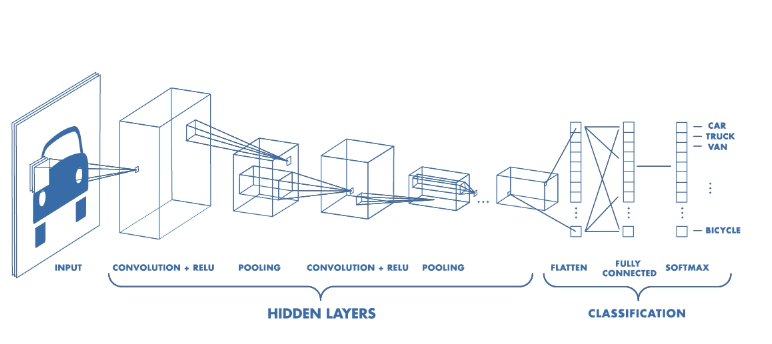
\includegraphics[width=0.8\textwidth]{fig/CNNExample.png}
    \caption{Exemplo clássico de uma arquitetura de CNN, mostrando a imagem de entrada, camadas convolucionais, camadas de pooling, camadas densas e saída.}
    \label{fig:cnnexample}
\end{figure} %imagem do google msm, nos livros parem mt complexas


% funcionamento e camadas imagem mapa de caracteristicas
O funcionamento das CNNs pode ser explicado em várias etapas. Primeiramente, a camada convolucional aplica filtros (ou kernels) aos dados de entrada. Esses filtros são pequenas matrizes que percorrem a imagem, realizando operações de convolução. Cada filtro é treinado para detectar diferentes características, como bordas, texturas e padrões específicos. A saída dessa operação é um mapa de características, que representa a presença dessas características na imagem original. O objetivo principal das camadas convolucionais é aprender a identificar e abstrair características relevantes dos dados de entrada, preservando as relações espaciais entre os pixels \cite{aggarwal2018neural}.

% pooling
Após a convolução, a saída passa por uma camada de pooling, que reduz a dimensionalidade dos mapas de características, mantendo as informações mais importantes. A camada de pooling mais comum é o max pooling, que seleciona o valor máximo de uma região específica do mapa de características. Esse processo ajuda a reduzir a quantidade de parâmetros e a computação na rede, além de tornar a detecção de características mais robusta a variações e deslocamentos na imagem \cite{aggarwal2018neural}.

% camadas densas
Finalmente, as camadas densas recebem a saída das camadas convolucionais e de pooling e produzem a saída final da rede. Nessas camadas, cada neurônio está conectado a todos os neurônios da camada anterior, permitindo a combinação e a interpretação das características extraídas. Como exemplo, pode-se observar uma CNN de quatro camadas com duas camadas densas na Figura \ref{fig:hiddenlayers}. As camadas densas são responsáveis por realizar a classificação final ou outras tarefas de saída \cite{nielsen2015neural}.

\begin{figure}
    \centering   
    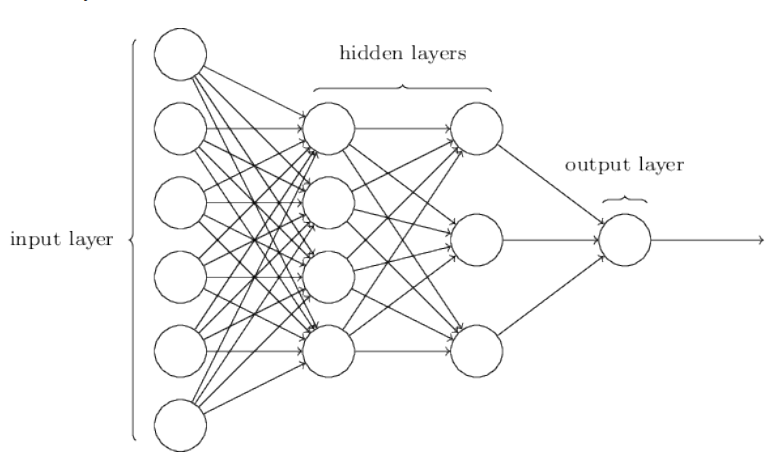
\includegraphics[width=0.8\textwidth]{fig/2hiddenlayers.png}
    \caption{Rede neural convolucional composta por uma camada de entrada, duas camadas densas e uma camada de saída.}
    \label{fig:hiddenlayers}
\end{figure}

% devo extender esse paragrafo? tem muita info eu achei
O treinamento das CNNs é realizado usando algoritmos de aprendizado supervisionado, como a retropropagação, em conjunto com otimizações como o gradiente descendente. Durante o treinamento, a rede ajusta os pesos dos filtros e das conexões entre os neurônios para minimizar a diferença entre a saída prevista e a saída desejada. A função de perda, que mede essa diferença, é calculada para cada exemplo do conjunto de treinamento, e os pesos são atualizados iterativamente para melhorar a precisão da rede \cite{aggarwal2018neural}.

As CNNs são especialmente poderosas devido à sua capacidade de capturar hierarquias de características, desde características de baixo nível, como bordas e texturas, até características de alto nível, como formas e objetos inteiros. Isso é conseguido através do empilhamento de múltiplas camadas convolucionais e de pooling, permitindo que a rede aprenda representações cada vez mais complexas dos dados de entrada \cite{goodfellow2016deep}.


Um exemplo clássico de CNN é a arquitetura LeNet-5, desenvolvida por Yann LeCun na década de 1990 para reconhecimento de dígitos manuscritos. Como pode ser visto na Figura \ref{fig:lenet5}, a LeNet-5 consiste em três camadas convolucionais seguidas por camadas de pooling, e termina com duas camadas totalmente conectadas. Essa arquitetura foi pioneira no uso de CNNs e demonstrou o potencial dessas redes para tarefas de visão computacional \cite{lecun1998gradient}.

\begin{figure}
    \centering   
    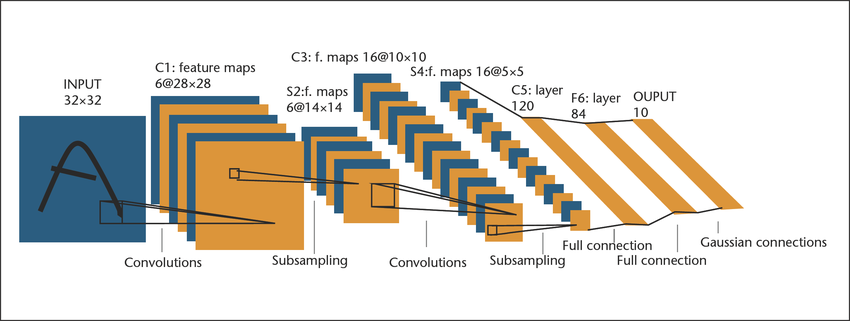
\includegraphics[width=\textwidth]{fig/A-Convolutional-Neural-Net-LeNet-5-From-Lecun-et-al-1998-C1998-IEEE-reprinted.png}
    \caption{Rede neural convolucional desenvolvida na década de 1990 por \citeonline{lecun1998gradient}.}
    \label{fig:lenet5}
\end{figure}


\section{Estimação de Profundidade}

% o que é

De acordo com \citeonline{khan2020deep}, o conceito de estimação de profundidade refere-se ao processo de preservar a informação tridimensional de uma cena a partir de informação bidimensional capturada por câmeras. Mapas de profundidade são imagens que caracterizam esse conceito, e podem ser representadas por imagens em escala de cinza onde os tons dos pixels são definidos de acordo com sua distância correspondente na cena original \cite{dourado2020multi}. 

\textcolor{red}{EXEMPLO DE MAPA DE PROFUNDIDADE}


%% como é capturado

Segundo \citeonline{rajapaksha2024deep}, as distâncias aos objetos em uma cena são percebidas pelos olhos humanos por meio de pistas visuais como o horizonte, pontos de fuga, tamanho relativo de objetos conhecidos, luz e sombra, e gradiente de textura.  



% Sensores RGBD - Red, Green, Blue, Depth - (Kinect v1, Kinect v2 (PAGLIARI;
% PINTO, 2015) e FARO Focus (VASILJEVIC et al., 2019)), Light Detection and Ranging
% (LiDAR), câmeras estéreo, Radio Detection And Ranging (RADAR) e Sound Navigation
% and Ranging (SONAR) são tecnologias que desempenham o papel de extrair dados de
% profundidade do ambiente e, além disso, são amplamente comercializadas. \cite{de2021aprendizagem}

Sensores de profundidade estão cada vez mais embarcados em equipamentos amplamente difundidos como dispositivos de realidade aumentada (Occulus, Kinect) e até mesmo em smartphones \cite{du2020depthlab}, principalmente as câmeras ToF, pois são capazes de desempenhar de maneira satisfatória mesmo com baixa potência \cite{branscombe2018microsoft}. De acordo com \cite{xie2021ultradepth}, a adoção de sensores de profundidade em smartphones tende a aumentar nos próximos anos, com diversas aplicações como tradução de linguagem de sinais \cite{park2021enabling} e sistemas de navegação mobile para pessoas com deficiência visual \cite{see2022smartphone}. 

Diversos tipos de técnicas são atualmente empregadas para adquirir informação de profundidade. Os métodos de aquisição de imagens de profundidade são divididos em duas categorias. Métodos ativos de estimação de profundidade envolvem calcular as distâncias interagindo fisicamente com os objetos do ambiente. Ultrassom e sensores \textit{Time of Flight} (ToF) por exemplo, utilizam da emissão de ondas com velocidade conhecida e medem o tempo de retorno a um receptor. Métodos passivos, por outro lado, envolvem a extração da informação através de processamento de imagens como visão estéreo e estimação monocular de profundidade \cite{khan2020deep}. 

De acordo com \citeonline{hansard2012time}, o funcionamento de câmeras ToF consiste em um emissor e um receptor de pulso de luz, a distância percorrida pode ser calculada medindo o atraso de detecção ou o desvio de fase do pulso recebido, produzindo um mapa de profundidade, como exemplificado na Figura \ref{fig:tof}. 

\begin{figure}[h]
    \centering   
    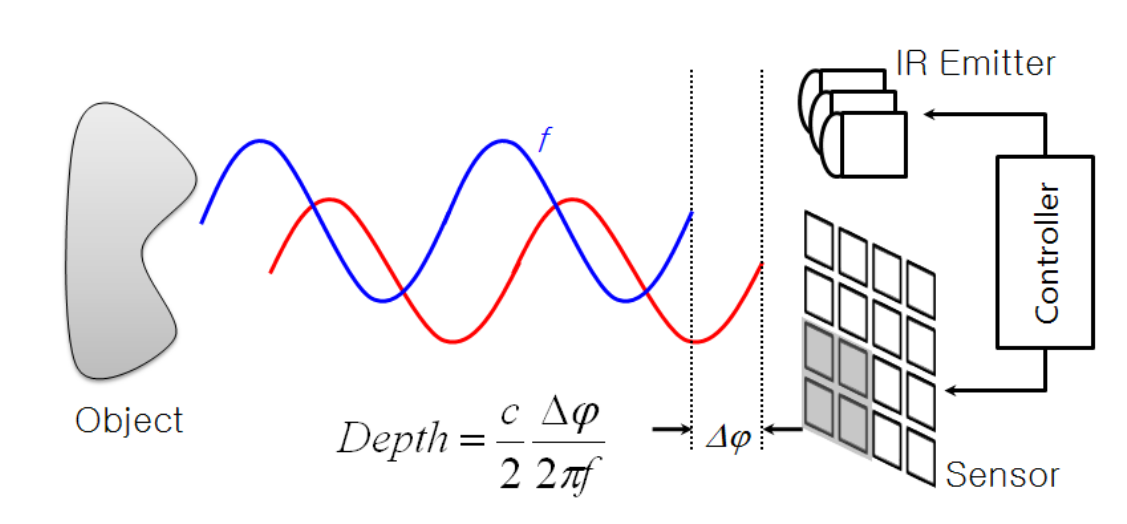
\includegraphics[width=0.8\textwidth]{fig/tof_cameras.png}
    \caption{Princípio de funcionamento de câmeras ToF. Fonte: \cite{hansard2012time}}
    \label{fig:tof}
\end{figure}

 O primeiro, chamado de ToF ponto-a-ponto, utiliza um mecanismo de inclinação panorâmica para obter uma sequência temporal de medições do tempo de retorno a cada ponto, essa técnica é conhecida como \textit{Light Detection and Ranging} (LiDAR). Esse tipo de técnica é empregada com maior frequência em sensoreamento em ambientes externos, por exemplo, sensores veiculares. Além disso, entre as vantagens desse tipo de tecnologia podemos citar a sua boa performance mesmo em cenários de baixa luminosidade ou em movimento e sua alta resolução e acurácia da informação adquirida \cite{zollhofer2019commodity}.


O segundo tipo é chamado de ToF modulado, em que uma câmera utiliza um pulso contínuo modulado em uma determinada frequência. A onda recebida é processada por um detector de desvio de fase. Um exemplo desse tipo de câmera é o Microsoft Kinect \cite{zollhofer2019commodity}.

De acordo com \citeonline{szeliski2022computer}, o termo correspondência estéreo (do inglês, \textit{Stereo Matching}) refere-se ao processo de construir um modelo 3D de uma cena por meio da busca de pixels correspondentes em pelo menos duas imagens 2D, convertendo assim, suas posições para o espaço de profundidade tridimensional. A técnica baseia-se na premissa de que o sistema visual humano percebe as profundidades através das diferenças entre as imagens capturadas pelos olhos esquerdo e direito. Segundo \citeonline{lahiri2024deep}, devido ao desenvolvimento da área do aprendizado profundo, atualmente, a técnica de estimação de profundidade por meio de visão estéreo é formulada por uma tarefa de aprendizado não-supervisionado.



Segundo \cite{castellano2023performance}, cada uma das técnicas de aquisição de imagens de profundidade possui lados negativos que podem impactar o seu emprego em aplicações práticas. Por exemplo, as câmeras ToF podem sofrer com invalidação de pixels próximos a cantos ou bordas de objetos devido à interferências entre os raios infravermelhos em superfícies descontínuas \cite{hansard2012time}. Outros tipos de câmeras RGB-D mais comuns podem produzir valores inválidos em superfícies muito brilhantes ou reflexivas como espelhos, superfícies metálicas ou muito escuras \cite{zollhofer2019commodity}. De acordo com \citeonline{zhang2022indepth} quando capturadas em ambientes internos, tais imagens podem conter até 50\% de dados faltantes \cite{zhang2018deep}. Dados de profundidade adquiridos por LiDAR não são densos, podendo chegar até 95\% de esparsidade, além do equipamento apresentar custo financeiro e energético elevado \cite{khan2020deep} \cite{hu2022deep}.


Compondo a lista de métodos passivos, a estimação de profundidade monocular refere-se ao processo de regredir um mapa de profundidade denso a partir de uma única imagem de câmera monocular \cite{birkl2023midas}. Segundo \citeonline{ranftl2020towards}, este ainda é um problema desafiador, visto que envolve a compreensão de pistas visuais, contexto de cenas e conhecimento prévio dos objetos para deduzir as relações geométricas da cena, o que implica na necessidade de técnicas baseadas em aprendizado. Com o desenvolvimento da área da inteligência artificial, técnicas mais robustas começaram a ser empregadas para estimação de profundidade. 


Segundo \citeonline{mertan2022single} um dos desafios que são intrínsecos ao problema de estimação monocular de profundidade é a ambiguidade. A partir de uma única imagem RGB podem haver um número muito grande de possíveis resultados 3D, ou seja, é caracterizado um problema de mapeamento onde cada entrada pode gerar muitas saídas. Por isso é considerado um problema mal-posto, ou do inglês, \textit{ill posed problem}.

